\section{Results and Discussion}
We focus on two questions: (1) Using domain-independent features indicative of the likelihood to reach $G_u$ from current state, can the intervening agent correctly interrupt to prevent the user from reaching $G_u$? and (2) How does the learning approach perform against state-of the-art plan/goal recognition? To address the first question, we evaluated the performance of the learned model to predict intervention on previously unseen problems.

The benchmark suite consists of Blocks-words, IPC Grid, Navigator and Ferry domains and the Generalized Rush Hour domain. For the Blocks-words domain, we chose word building problems. The words user and the attacker want to build are different but they have some common letters (e.g., TAD/BAD). The attacker is able to exploit the user's progress on stacking blocks to complete word the attacker wants to build. In the IPC grid domain, an agent moves through a grid to get from point A to B. Certain locked positions on the grid can be opened by picking up keys. In the Navigator domain, an agent simply moves from one point in grid to another. In the Ferry domain, a single ferry moves cars between different locations. In Easy-IPC and Navigator domains, we designated certain locations on the grid as traps. The goal of the robot is to navigate to a specific point on the grid safely. In the Ferry domain a port is \emph{compromised} and a ferry carrying a car there results in an undesirable state. The ferry's objective is to transport cars to specified locations without passing a compromised port. In the Rush Hour domain, we created puzzles containing vehicles that need not be moved on arbitrary grid sizes and exits. Intervention is generated when the user moves any of the forbidden vehicles while solving the puzzle.

We generate 3 separate test instances of 20 problems each (total of 60) for the benchmark domains containing problems different from trained instances. For example, number of blocks in the domain (block-words), size of grid (navigator, easy-ipc), accessible and inaccessible paths on the grid (navigator, easy-ipc), properties of artifacts in the grid (easy-ipc). For each problem in an instance we generated 10 observation traces (total of 600 test observation traces). For the Rush Hour domain we created 2200 observation traces and split to training and testing 60/40. We define true-positive as the classifier correctly predicting (Y). True-negative is an instance where the classifier  correctly predicts (N). False-positives are instances where classifier incorrectly predicts an observation as an interrupt. False-negatives are instances where the classifier incorrectly predicts the observation not as an interrupt. We report precision (P), recall (R) and F1-Measure (F1).

\begin{table*}[tb]
\resizebox{\textwidth}{!}{%
\begin{tabular}{|l|lllllllll|lllllllll|lllllllll|lllllllll|}
\hline
\multicolumn{1}{|c|}{\multirow{3}{*}{\textbf{Domain}}} & \multicolumn{9}{c|}{\textbf{Naive Bayes}} & \multicolumn{9}{c|}{\textbf{Decision Tree}} & \multicolumn{9}{c|}{\textbf{Logistic Regression}} & \multicolumn{9}{c|}{\textbf{K-Nearest}} \\ \cline{2-37} 
\multicolumn{1}{|c|}{} & \multicolumn{3}{c|}{\textbf{Inst 1}} & \multicolumn{3}{c|}{\textbf{Inst 2}} & \multicolumn{3}{c|}{\textbf{Inst 3}} & \multicolumn{3}{c|}{\textbf{Inst 1}} & \multicolumn{3}{c|}{\textbf{Inst 2}} & \multicolumn{3}{c|}{\textbf{Inst 3}} & \multicolumn{3}{c|}{\textbf{Inst 1}} & \multicolumn{3}{c|}{\textbf{Inst 2}} & \multicolumn{3}{c|}{\textbf{Inst 3}} & \multicolumn{3}{c|}{\textbf{Inst 1}} & \multicolumn{3}{c|}{\textbf{Inst 2}} & \multicolumn{3}{c|}{\textbf{Inst 3}} \\ \cline{2-37} 
\multicolumn{1}{|c|}{} & \multicolumn{1}{c|}{P} & \multicolumn{1}{c|}{R} & \multicolumn{1}{c|}{F1} & \multicolumn{1}{l|}{P} & \multicolumn{1}{l|}{R} & \multicolumn{1}{l|}{F1} & \multicolumn{1}{l|}{P} & \multicolumn{1}{l|}{R} & F1 & \multicolumn{1}{l|}{P} & \multicolumn{1}{l|}{R} & \multicolumn{1}{l|}{F1} & \multicolumn{1}{l|}{P} & \multicolumn{1}{l|}{R} & \multicolumn{1}{l|}{F1} & \multicolumn{1}{l|}{P} & \multicolumn{1}{l|}{R} & F1 & \multicolumn{1}{l|}{P} & \multicolumn{1}{l|}{R} & \multicolumn{1}{l|}{F1} & \multicolumn{1}{l|}{P} & \multicolumn{1}{l|}{R} & \multicolumn{1}{l|}{F1} & \multicolumn{1}{l|}{P} & \multicolumn{1}{l|}{R} & F1 & \multicolumn{1}{l|}{P} & \multicolumn{1}{l|}{R} & \multicolumn{1}{l|}{F1} & \multicolumn{1}{l|}{P} & \multicolumn{1}{l|}{R} & \multicolumn{1}{l|}{F1} & \multicolumn{1}{l|}{P} & \multicolumn{1}{l|}{R} & F1 \\ \hline
\multicolumn{37}{|c|}{\textbf{Full Method}} \\ \hline
\textbf{Blocks} & 1 & 1 & 1 & 1 & 1 & 1 & 1 & 1 & 1 & 1 & 1 & 1 & 1 & 1 & 1 & 1 & 1 & 1 & 1 & 1 & 1 & 1 & 1 & 1 & 1 & 1 & 1 & 1 & 1 & 1 & 1 & 1 & 1 & 1 & 1 & 1 \\ \cline{1-1}
\textbf{EasyIPC} & 1 & 1 & 1 & 1 & 1 & 1 & 1 & 1 & 1 & 1 & 1 & 1 & 1 & 1 & 1 & 1 & 1 & 1 & .78 & 1 & .88 & .78 & 1 & .88 & .76 & 1 & .86 & 1 & 1 & 1 & 1 & 1 & 1 & 1 & 1 & 1 \\ \cline{1-1}
\textbf{Ferry} & 1 & 1 & 1 & 1 & 1 & 1 & 1 & 1 & 1 & 1 & 1 & 1 & 1 & 1 & 1 & 1 & 1 & 1 & 1 & 1 & 1 & 1 & 1 & 1 & 1 & 1 & 1 & 1 & 1 & 1 & 1 & 1 & 1 & 1 & 1 & 1 \\ \cline{1-1}
\textbf{Navigator} & 1 & 1 & 1 & 1 & 1 & 1 & 1 & .9 & .9 & .76 & 1 & .87 & .56 & 1 & .72 & .82 & 1 & .9 & 1 & 1 & 1 & 1 & 1 & 1 & .99 & 1 & .99 & 1 & 1 & 1 & .92 & 1 & .96 & .99 & 1 & .99 \\ \hline
\multicolumn{37}{|c|}{\textbf{Partial Method}} \\ \hline
\textbf{Blocks} & .14 & 1 & .25 & .14 & 1 & .25 & .14 & 1 & .25 & .14 & 1 & .25 & .14 & 1 & .25 & .14 & 1 & .25 & .14 & 1 & .25 & .14 & 1 & .25 & .14 & 1 & .25 & 1 & 1 & 1 & 1 & 1 & 1 & 1 & 1 & 1 \\ \cline{1-1}
\textbf{EasyIPC} & 1 & 1 & 1 & 1 & 1 & 1 & 1 & 1 & 1 & 1 & 1 & 1 & 1 & 1 & 1 & 1 & 1 & 1 & .79 & .54 & .64 & .36 & .62 & .45 & .71 & .63 & .67 & .04 & .06 & .05 & .03 & .07 & .05 & 0.04 & .08 & .05 \\ \cline{1-1}
\textbf{Ferry} & .28 & .45 & .34 & .22 & .6 & .32 & .01 & .06 & .02 & .15 & .62 & .25 & .15 & .57 & .24 & .9 & .82 & .86 & .21 & .54 & .3 & .17 & .57 & .23 & 1 & 1 & 1 & .2 & .89 & .33 & .07 & .1 & .13 & 1 & .67 & .8 \\ \cline{1-1}
\textbf{Navigator} & 1 & 1 & 1 & 1 & 1 & 1 & 1 & 1 & 1 & .45 & 1 & .62 & 1 & 1 & 1 & 1 & 1 & 1 & .51 & .72 & .6 & .97 & 1 & .98 & .95 & 1 & .97 & .45 & 1 & .62 & 1 & 1 & 1 & 1 & 1 & 1 \\ \cline{1-1}
\textbf{Rush Hour} & .43 & .45 & .44 & \multicolumn{6}{l|}{} & .9 & .88 & .89 & \multicolumn{6}{l|}{} & .63 & .51 & .56 & \multicolumn{6}{l|}{} & .93 & .85 & .89 & \multicolumn{6}{l|}{} \\ \hline
\end{tabular}%
}
\caption{Precision (P),Recall (R),F1 measures for predicting intervention in Full and Parial methods}
\label{tab:exactapprox}
\end{table*}

\begin{table*}[tb]
\small
\resizebox{\textwidth}{!}{%
\begin{tabular}{|l|lllllllll|lllllllll|lllllllll|}
\hline
\multicolumn{1}{|c|}{\multirow{3}{*}{\textbf{Domain}}} & \multicolumn{9}{c|}{\textbf{Inst 1}} & \multicolumn{9}{c|}{\textbf{Inst 2}} & \multicolumn{9}{c|}{\textbf{Inst 3}} \\ \cline{2-28} 
\multicolumn{1}{|c|}{} & \multicolumn{3}{l|}{RG (LAMA)} & \multicolumn{3}{l|}{RG (HSP)} & \multicolumn{3}{c|}{GM} & \multicolumn{3}{c|}{RG (LAMA)} & \multicolumn{3}{c|}{RG (HSP)} & \multicolumn{3}{c|}{GM} & \multicolumn{3}{c|}{RG (LAMA)} & \multicolumn{3}{c|}{RG (HSP)} & \multicolumn{3}{c|}{GM} \\ \cline{2-28} 
\multicolumn{1}{|c|}{} & \multicolumn{1}{c|}{P} & \multicolumn{1}{c|}{R} & \multicolumn{1}{c|}{F1} & \multicolumn{1}{l|}{P} & \multicolumn{1}{l|}{R} & \multicolumn{1}{l|}{F1} & \multicolumn{1}{l|}{P} & \multicolumn{1}{l|}{R} & F1 & \multicolumn{1}{l|}{P} & \multicolumn{1}{l|}{R} & \multicolumn{1}{l|}{F1} & \multicolumn{1}{l|}{P} & \multicolumn{1}{l|}{R} & \multicolumn{1}{l|}{F1} & \multicolumn{1}{l|}{P} & \multicolumn{1}{l|}{R} & F1 & \multicolumn{1}{l|}{P} & \multicolumn{1}{l|}{R} & \multicolumn{1}{l|}{F1} & \multicolumn{1}{l|}{P} & \multicolumn{1}{l|}{R} & \multicolumn{1}{l|}{F1} & \multicolumn{1}{l|}{P} & \multicolumn{1}{l|}{R} & F1 \\ \hline
\textbf{Blocks} & .23 & 1 & .38 & .23 & 1 & .38 & .22 & 1 & .36 & .27 & 1 & .43 & .27 & 1 & .43 & .24 & 1 & .39 & .25 & 1 & .4 & .25 & 1 & .4 & .24 & 1 & .38 \\ \cline{1-1}
\textbf{EasyIPC} & .24 & 1 & .39 & .1 & .19 & .13 & .1 & .19 & .11 & .13 & .47 & .21 & .12 & .38 & .18 & .1 & .24 & .12 & .15 & .45 & .23 & .13 & .45 & .23 & .1 & .39 & .14 \\ \cline{1-1}
\textbf{Ferry} & .1 & .49 & .17 & .18 & .29 & .22 & .1 & .1 & .1 & .13 & .73 & .22 & .1 & .13 & .11 & - & 0 & - & .1 & .44 & .14 & .85 & .32 & .47 & - & 0 & 1 \\ \cline{1-1}
\textbf{Navigator} & - & 0 & - & - & 0 & - & - & 0 & - & - & 0 & - & - & 0 & - & - & 0 & - & - & 0 & - & - & 0 & - & - & 0 & - \\ \hline
\end{tabular}%
}
\caption{Precision (P),Recall (R),F1 measures for recognizing intervention with probabilistic plan recognition (RG) using a satisficing (LAMA) and optimal (HSP) planners and goal mirroring (GM). P=-,R=0,F1=- means the true-negative, false negative rates were 100\%  each}
\label{tab:rgv}
\end{table*}

To test what existing plan/goal recognition algorithms can recognize the user's goal/plan in time and accurately, we implemented Ramirez and Geffener's probabilistic plan recognition algorithm \cite{ramirez2010probabilistic} and the Goal Recognition algorithm in Vered et al. \shortcite{vered2018goalrec}. Both approaches rank the goal hypotheses ($G_u$ and $G_d$ in the intervention problem) according to a probability distribution $P(G|O)$ where $O$ is the observation sequence. Vered et al. first prune the goal hypotheses using landmarks and then rank the remaining goal. As each observation is made available, the observer repeatedly solves each approach. If $G_u$ is the top ranked goal when an actual unsafe action observed, intervention will be triggered (true positive). We used the same test data suite to evaluate accuracy.

Table \ref{tab:exactapprox} shows that the classifiers trained with Full method achieve very high precision and recall for all the domains when predicting intervention. Low false positives and false negatives suggests that the user will not be unnecessarily interrupted. As expected performance degrades with the Partial method. For the benchmark domains we were able to discover at least one classifier responded with very high precision and recall with the plan similarity features, the exception being the Ferry domain. 
The Rush Hour domain produced comparatively better results, with the decision tree and K-Nearest neighbor classifiers being the best. 

The plan similarity features do not sufficiently capture criticality of the state as opposed to  the Full method. Full method features accurately separates instances where the user has limited/no options available to reach the desirable goal while avoiding the undesirable state. Thus the classifiers perform well in recognizing critical actions in new problems. Plan similarity features rely on the learning algorithm to produce better output when predicting intervention. 

Comparing with results in Table \ref{tab:rgv}, we see that learning methods outperform adaptations of existing plan/goal recognition algorithms to predict intervention. P=-,R=0,F1=- means the true-negative, false negative rates were 100\%  each (i.e., many observations that should have been identified as critical actions were missed). The algorithms we selected clearly struggled to predict intervention in the Navigator domain. This allows us to conclude that although plan cost  metrics perform well in recognizing goals/plans, they often fail to predict intervention because in intervention, time point at which recognition occurs matters. If recognition is delayed, many false negatives occur while early recognition results in false alarms.


%\section{Explaining Intervention}
%When the classifier predicts intervention we want the user to be able to trust the prediction to accept it. Interpretability of the model instills trust \cite{ribeiro2016}. We rely on Miller's definition of interpretability: ``Interpretability is the degree to which an observer can understand the cause of a decision''\cite{miller2017}. The four classifiers were selected for their ability to produce interpretable models for domains similar to medical diagnosis \cite{gallego2015,sun2005,friedler2019,craven1995}. Although the interpretable classifier itself can explain the prediction (Ribeiro et al. 2016) \nocite{ribeiro2016}, we focus on explaining causality of intervention.
%
%The general structure of a causality in planning can be defined as $x \xrightarrow py$ where $x$ and $y$ are actions (or events) and $x$ occurs before $y$ and $p$ is a proposition representing an effect of $x$ and a precondition of $y$. No event takes between $x$ and $y$ place that adds $\neg p$.
%
%In the approximate method, the observer builds a reference plan that is compatible with the observations. We implemented the algorithm by Ambite and Knoblock\shortcite{ambite2001} that converts a total order plan to partial order plans. Given the reference plan compatible with observations, the algorithm produces the partially ordered causal structures consistent with the input plan. We then use these partial orders to reason about intervention. Causal structure for the reference plan when $G_u=$BAD in the blocks world domain is shown in Figure \ref{fig:causal}. When an observation occurs in the domain, the observer uses the causal structure to provide answers to: (1) which predicates did the most recent observation enable, (2) which predicates have been enabled so far, (3) which predicates are required for the undesirable state, and (4) which actions should take place to reach undesirable state from current state.
%
%\begin{figure}[tb]
%	\centering{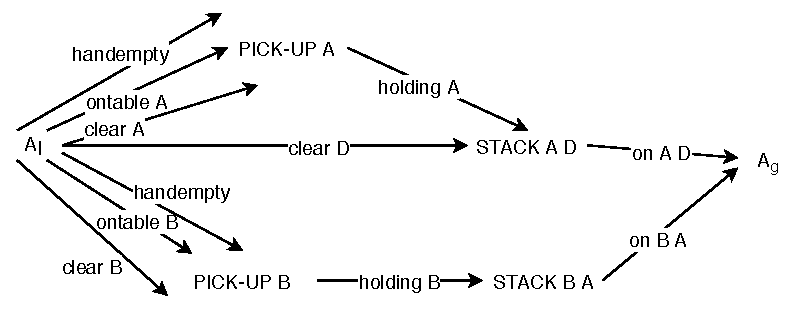
\includegraphics[width=\columnwidth]{causal.pdf}}
%	\caption{Causal structure for an observation compatible plan in blocks words domain. $A_I$ and $A_g$ are dummy actions indicating initial and goal states respectively}
%	\label{fig:causal}
%\end{figure}
%
%To answer question 1, the observer searches through the causal structure to find the action node for the current observation (e.g., breadth-first search). Causal edges leaving the node are the predicates that the observation has enabled. For example, in Figure \ref{fig:causal} observation PICK-UP A enables predicate HOLDING A. To answer question 2, we find all paths between $A_I$ and the most recent observation in the causal structure. Predicates that have been made active by observations can be found by unifying the found paths. The answer to question 3 are the edges incident on $A_g$. To answer question 4, we find all paths between the most recent observed action and $A_g$. Once the observer flags an observation as requiring intervention, it produces the following statement template as an explanation: \textit{Undesirable state is immediately reachable by [current observation]. Observation enables [answer to question 1]. Current state [answer to question 2] leads to the undesirable state by enabling [answer to question 4]. Undesirable state is satisfied by [answer to question 3]}. We are currently evaluating these explanations in a human user study.